
%%%%%%%%%%%%%%%%%%%%%%%%%%%%%%%%%%%%%%%%%%%%%%%%%%%%%%%%%%%%%%%%%%%%%
%% This is a (brief) model paper using the achemso class
%% The document class accepts keyval options, which should include
%% the target journal and optionally the manuscript type.
%%%%%%%%%%%%%%%%%%%%%%%%%%%%%%%%%%%%%%%%%%%%%%%%%%%%%%%%%%%%%%%%%%%%%
\documentclass[journal=jacsat,manuscript=article]{achemso}

%%%%%%%%%%%%%%%%%%%%%%%%%%%%%%%%%%%%%%%%%%%%%%%%%%%%%%%%%%%%%%%%%%%%%
%% Place any additional packages needed here.  Only include packages
%% which are essential, to avoid problems later. Do NOT use any
%% packages which require e-TeX (for example etoolbox): the e-TeX
%% extensions are not currently available on the ACS conversion
%% servers.
%%%%%%%%%%%%%%%%%%%%%%%%%%%%%%%%%%%%%%%%%%%%%%%%%%%%%%%%%%%%%%%%%%%%%
%%\usepackage[version=3]{mhchem} % Formula subscripts using \ce{}
\usepackage[T1]{fontenc}       % Use modern font encodings
\usepackage{hyperref}

\usepackage{xcolor}

%%%%%%%%%%%%%%%%%%%%%%%%%%%%%%%%%%%%%%%%%%%%%%%%%%%%%%%%%%%%%%%%%%%%%
%% If issues arise when submitting your manuscript, you may want to
%% un-comment the next line.  This provides information on the
%% version of every file you have used.
%%%%%%%%%%%%%%%%%%%%%%%%%%%%%%%%%%%%%%%%%%%%%%%%%%%%%%%%%%%%%%%%%%%%%
%%\listfiles

%%%%%%%%%%%%%%%%%%%%%%%%%%%%%%%%%%%%%%%%%%%%%%%%%%%%%%%%%%%%%%%%%%%%%  
%% Place any additional macros here.  Please use \newcommand* where
%% possible, and avoid layout-changing macros (which are not used
%% when typesetting).
%%%%%%%%%%%%%%%%%%%%%%%%%%%%%%%%%%%%%%%%%%%%%%%%%%%%%%%%%%%%%%%%%%%%%
\newcommand*\mycommand[1]{\texttt{\emph{#1}}}
\newcommand*\fref[1]{Figure~\ref{fig:#1}}
\newcommand*\tref[1]{Table~\ref{table:#1}}
\newcommand*\sref[1]{Section~\ref{sec:#1}}
\newcommand*\eg{e.g.~}
\newcommand*\ie{i.e.~}
%\newcommand*\citeauthoryear[1]{{\citeauthor{#1}~(\citeyear{#1})}}

%%%%%%%%%%%%%%%%%%%%%%%%%%%%%%%%%%%%%%%%%%%%%%%%%%%%%%%%%%%%%%%%%%%%%
%% Meta-data block
%% ---------------
%% Each author should be given as a separate \author command.
%%
%% Corresponding authors should have an e-mail given after the author
%% name as an \email command. Phone and fax numbers can be given
%% using \phone and \fax, respectively; this information is optional.
%%
%% The affiliation of authors is given after the authors; each
%% \affiliation command applies to all preceding authors not already
%% assigned an affiliation.
%%
%% The affiliation takes an option argument for the short name.  This
%% will typically be something like "University of Somewhere".
%%
%% The \altaffiliation macro should be used for new address, etc.
%% On the other hand, \alsoaffiliation is used on a per author basis
%% when authors are associated with multiple institutions.
%%%%%%%%%%%%%%%%%%%%%%%%%%%%%%%%%%%%%%%%%%%%%%%%%%%%%%%%%%%%%%%%%%%%%
\author{Deepak Bandyopadhyay}
\email{deepak.2.bandyopadhyay@gsk.com}
\author{Constantine Kreatsoulas}
\author{Pat G. Brady}
\author{Joseph Boyer}
\author{Zangdong He}
\author{Genaro Scavello Jr.}
\affiliation[GSK]{GlaxoSmithKline, 1250 S. Collegeville Rd, Collegeville, PA 19426}
\author{Dac-Trung Nguyen}
\author{Tyler Peryea}
\author{Rajarshi Guha}
\email{guhar@mail.nih.gov}
\author{Ajit Jadhav}
\email{ajadhav@mail.nih.gov}
%\phone{+123 (0)123 4445556}
%\fax{+123 (0)123 4445557}
\affiliation[NCATS]{National Center for Advancing Translational Science, 9800 Medical Center Drive, Rockville, MD 20850}

%%%%%%%%%%%%%%%%%%%%%%%%%%%%%%%%%%%%%%%%%%%%%%%%%%%%%%%%%%%%%%%%%%%%%
%% The document title should be given as usual. Some journals require
%% a running title from the author: this should be supplied as an
%% optional argument to \title.
%%%%%%%%%%%%%%%%%%%%%%%%%%%%%%%%%%%%%%%%%%%%%%%%%%%%%%%%%%%%%%%%%%%%%
\title[Scaffold Analytics] {Scaffold-Based Analytics: Enabling Hit-to-Lead
  Decisions by Visualizing Chemical Series Linked Across Large Datasets}  

%%%%%%%%%%%%%%%%%%%%%%%%%%%%%%%%%%%%%%%%%%%%%%%%%%%%%%%%%%%%%%%%%%%%%
%% Some journals require a list of abbreviations or keywords to be
%% supplied. These should be set up here, and will be printed after
%% the title and author information, if needed.
%%%%%%%%%%%%%%%%%%%%%%%%%%%%%%%%%%%%%%%%%%%%%%%%%%%%%%%%%%%%%%%%%%%%%
%\abbreviations{IR,NMR,UV}
%\keywords{American Chemical Society, \LaTeX}

%%%%%%%%%%%%%%%%%%%%%%%%%%%%%%%%%%%%%%%%%%%%%%%%%%%%%%%%%%%%%%%%%%%%%
%% The manuscript does not need to include \maketitle, which is
%% executed automatically.
%%%%%%%%%%%%%%%%%%%%%%%%%%%%%%%%%%%%%%%%%%%%%%%%%%%%%%%%%%%%%%%%%%%%%
\begin{document}

%%%%%%%%%%%%%%%%%%%%%%%%%%%%%%%%%%%%%%%%%%%%%%%%%%%%%%%%%%%%%%%%%%%%%
%% The "tocentry" environment can be used to create an entry for the
%% graphical table of contents. It is given here as some journals
%% require that it is printed as part of the abstract page. It will
%% be automatically moved as appropriate.
%%%%%%%%%%%%%%%%%%%%%%%%%%%%%%%%%%%%%%%%%%%%%%%%%%%%%%%%%%%%%%%%%%%%%
\begin{tocentry}

Some journals require a graphical entry for the Table of Contents.
This should be laid out ``print ready'' so that the sizing of the
text is correct.

Inside the \texttt{tocentry} environment, the font used is Helvetica
8\,pt, as required by \emph{Journal of the American Chemical
Society}.

The surrounding frame is 9\,cm by 3.5\,cm, which is the maximum
permitted for  \emph{Journal of the American Chemical Society}
graphical table of content entries. The box will not resize if the
content is too big: instead it will overflow the edge of the box.

This box and the associated title will always be printed on a
separate page at the end of the document.

\end{tocentry}

%%%%%%%%%%%%%%%%%%%%%%%%%%%%%%%%%%%%%%%%%%%%%%%%%%%%%%%%%%%%%%%%%%%%%
%% The abstract environment will automatically gobble the contents
%% if an abstract is not used by the target journal.
%%%%%%%%%%%%%%%%%%%%%%%%%%%%%%%%%%%%%%%%%%%%%%%%%%%%%%%%%%%%%%%%%%%%%
\begin{abstract}
  We present a method for visualizing and navigating large and diverse
  chemical spaces, such as screening datasets, along with their
  activities and properties. Our approach is to annotate the data with
  all possible scaffolds contained within each molecule using an
  exhaustive algorithm developed at NCATS.  We have developed a
  Spotfire visualization, coupled to a fuzzy clustering approach, that
  is used to drive the hit triage process. Progression decisions can
  be made using aggregate scaffold parameters and data from multiple
  datasets merged at the scaffold level.  This visualization easily
  reveals overlaps that help prioritize hits, highlight tractable
  series and posit ways to combine aspects of multiple hits.  The SAR
  of a large and complex hit is automatically mapped into all
  constituent scaffolds making it possible to navigate, via any shared
  scaffold, to all related hits.  This scaffold ``walking'' helps
  address bias toward a handful of potent and ligand-efficient
  molecules at the expense of coverage of chemical space. The mapping
  also automates the laborious process of substructure searches within
  a dataset as structures are now linked to pre-processed search
  results.  We compare the NCATS scaffold generation method with
  published screening triage methods such as nearest-neighbor
  clustering, data-driven clustering and scaffold
  networks. \textbf{\textcolor{red}{Can you add a line here that
      summarizes how this method turns out better than these
      pre-existing methods?}}  The workflow of a Spotfire
  visualization used in combination with fuzzy clustering and
  structure annotation provides a novel view of large and diverse
  datasets. This allows teams to effortlessly navigate between
  structurally related molecules and enriches the population of leads
  considered and progressed in a manner complementary to established
  approaches.
\end{abstract}

%%%%%%%%%%%%%%%%%%%%%%%%%%%%%%%%%%%%%%%%%%%%%%%%%%%%%%%%%%%%%%%%%%%%%
%% Start the main part of the manuscript here.
%%%%%%%%%%%%%%%%%%%%%%%%%%%%%%%%%%%%%%%%%%%%%%%%%%%%%%%%%%%%%%%%%%%%%
\section{Introduction}

The advantage and disadvantage of high throughput screening (HTS)
campaigns is the large amount of data that is generated. While the
value of large scale HTS has been debated\cite{Macarron:2011qv}, the
massive structure-activity datasets generated create a challenge in
identifying truly active compounds and their analogs and weeding out
false positives. The process of reducing HTS datasets from hundreds of
thousands of compounds to a few thousand or hundred active series is
termed triaging. Over the last twenty years many approaches to HTS
triaging have been described which include activity based
thresholds\cite{Mulrooney:2013aa}, similarity to known
actives\cite{Shanmugasundaram:2005aa}, enrichment based
approaches\cite{Varin2010CSE,Pu:2012wf}, ranges of physicochemical
properties\cite{Cox:2012qy}, crowdsourcing\cite{Peng:2013qp} and
removal of promiscuous or otherwise undesirable chemotypes
\cite{Dahlin:2014fp}. See \citeauthor{Shun:2011sy} and
\citeauthor{Langer:2009mw} for a review of HTS triage approaches.

One of the key challenges in the triage step is to identify structure-activity
series - sets of compounds with similar or analogous structures that exhibit a
spectrum of activity, including lack of activity. Identifying such subsets allows one to have some
confidence in the presence of a structure-activity relationship amongst the
active compounds which enables a more efficient exploration of the chemical
space around the selected hits. A good review of computational methods to extract SAR from screening datasets can be found in \citeauthor{Wawer2010review}. 

Given that a SAR series is, ideally, defined in terms of a core structure along
with various decorations, a natural first step in the triage process is to
identify these core structures, termed scaffolds. Usually this starts by
decomposing the structures in the screening collection, either exhaustively or
else using one of the many methods to decompose structures into fragments such
as the Bemis-Murcko\cite{BemisMurcko1999,BemisMurcko1996} or RECAP
methods\cite{Lewell:1998aa}. These methods lead to a large number of
fragments ranging from trivial ones such as a benzene ring to very complex
multiring structures. Thus a key step involves identifying the \emph{relevant} set of
scaffolds and their associated compounds. This can be challenging since a given
compound can contain multiple scaffolds and which scaffolds are
deemed relevant can be a subjective decision\cite{Hu:2016aa}.

In this work we present a HTS triage workflow based on navigating the
scaffold-activity landscape of a screening collection using a fuzzy clustering method to group compounds 
based on scaffold membership. The workflow includes
methods to visualize the activity landscape as well as methods to explore
different regions of chemical space via shared scaffolds. We also highlight the
efficiency gains obtained by using pre-computed scaffold associations rather
than performing substructure searches on the fly.

\subsection{Related Work}
While there are many ways to generate a set of scaffolds from a
compound collection, a key step is to identify a
relevant subset of them or else aggregate them in a way that leads to a useful
clustering of active and inactive compounds. While the term ``useful'' is rather
subjective, it is easy to identify cases that are \emph{not} useful. Thus, 5- or
6-member undecorated rings are likely not useful since they will occur in the
majority of compounds in a screening collection. At the other extreme, large,
extended scaffolds that are associated with very few compounds are also likely
not useful.

As a result, many approaches to scaffold aggregation have been described. A
natural approach is to consider a hierarchical aggregation. The Scaffold
Tree\cite{Ertl2011ScaffoldTree} and Scaffold Network\cite{Varin2011ScafNet}
define a hierarchical decomposition from more specialized larger scaffolds to
more inclusive smaller scaffolds. While the Scaffold Tree splits each larger
scaffold in exactly one way into two scaffolds with fewer rings, the Scaffold
Network performs an exhaustive decomposition into all possible smaller scaffolds
with fewer rings.  Since some subscaffolds are shared with neighboring
scaffolds, this produces a network or graph rather than a tree. The Scaffold
Network Generator program\cite{Matlock2013SNG} is a fast, easy-to-use public
command line implementation of Scaffold Networks that can scale to millions of
compounds via aggregation of scaffolds from split datasets and parallel
execution.  \citeauthor{Harper2004DDclus} use exhaustive enumeration to find all
Bemis-Murcko like frameworks in each molecule, and then recursively retain those
frameworks with highest aggregate activity and remove molecules that contain
them until a threshold is met, yielding a set of disjoint frameworks.  Other
methods have used multiple common substructure (MCS), first proposed for finding
protein structural similarity\cite{Koch1997MCSprot}, for example
\citeauthor{Quintus2009MCS} and the ChemAxon product LibraryMCS. 

To overcome the effect of small variations in heteroatoms (eg. O to S) mapping
otherwise similar molecules to different scaffolds, generalized or consolidated
scaffold representations have been proposed, such as the Reduced
Graph\cite{Barker2003RG}, the Bemis-Murcko scaffold\cite{BemisMurcko1996} and
the topological or 2D pharmacophore\cite{Schneider1999ScafHopTP}. Bemis-Murcko
like frameworks \cite{Harper2004DDclus} are generalized Bemis-Murcko scaffolds
where atom types and/or bond orders may be retained.

Multiple scaffolds if present in a dataset can be inferred from the
scaffold tree decomposition\cite{ClarkLabute2008SAReport}. However in
practice, the thresholds used by \citeauthor{ClarkLabute2008SAReport}
miss common scaffolds in HTS-like diverse chemical compound
sets. \citeauthor{Bandyopadhyay2011ACS} have used a common fragment
decomposition plug-in for SAReport in order to find and export
scaffolds for diverse datasets, such as the GSK Natural Products
Set\cite{Coma2014}.  This approach assigns at most one scaffold for
each molecule, based on the order they are selected by the user from a
prioritized list.

\begin{figure}
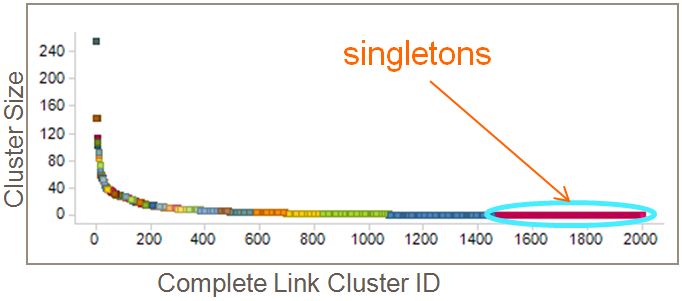
\includegraphics[width=5.5in]{fig/singletons.png}
\caption{Singletons in a complete-linkage clustering of the TCAMS dataset.}
\label{fig:platypus}
\end{figure}

Assigning each molecule to a single group partitions the dataset into
disparate, non-overlapping groups (also termed a hard clustering).
This is also the way most fingerprint-based agglomerative clustering
methods such as sphere exclusion, single and complete linkage
clustering work\cite{Downs2003}. On the other hand, it may be the case
that a molecule could well be assigned simultaneously to multiple
clusters, depending on the structural features present. Traditional
hard clustering methods will not allow this and as a result will tend
to assign such molecules to their own cluster, thus identifying them
as singletons, Such a result can be observed in real chemical datasets
as well -- for example, the complete-linkage clustering of the TCAMS
dataset\cite{Gamo2010,Calderon2011} has nearly 25\% of the 2000
clusters containing just one compound, as shown in \fref{platypus}.

In contrast to these partitioning clusters, the methods described
herein rely on fuzzy clustering, where a molecule may be assigned to
multiple clusters. Fuzzy clusters have been rarely used in
cheminformatics (for example \cite{Holliday2004,Richmond2015Galois}),
perhaps because they are hard to visualize and navigate.  In this work
we provide an intuitive visual framework that we believe can help end
users easily navigate a diverse chemical dataset describd by a fuzzy
clustering of multiple overlapping scaffolds per molecule.

\subsection{Datasets}
\label{sec:datasets}
The datasets used to illustrate and visualize our methods were picked
to represent the kinds of screening datasets we expect the method to
be used on in practice. For example, the TCAMS dataset\cite{Gamo2010}
consists of 13.5k diverse hits from an antimalarial screen at GSK,
along with pIC50 against a susceptible strain of the malarial parasite
(3D7), percentage inhibition against a resistant strain (DD2), Hep G2
hepatotoxicity, a few physical chemical properties (\eg molecular
weight, aromatic ring count, cLogP), and Inhibition Frequency Index
(IFI, a measure of promiscuity defined as the percentage of screens in
which a molecule inhibits over 50\%, \cite{Chakravorty2013IFI}).

The in-house kinase dataset shown, by contrast, is perhaps less
diverse but chosen to illustrate the power of this approach in joining
and merging datasets from multiple screens, combining their SAR to
design hybrid molecules, and making inferences about unknown activity
in one screen based on known activity in another screen.

These two and our other datasets are tabulated in \tref{dataset}, with
references provided where available.

Next, we describe several methods we have assembled as part of our
workflow that enable multiple scaffolds to be assigned to each
molecule and easy navigation between molecules related by these
scaffolds.


%\begin{itemize}
%\item Scaffold decomposition algorithm, description
%\subitem Comparison with other decomposition algorithms
%\item Linking R-group tool to Spotfire
%\item Developing the Spotfire vis UI
%\end{itemize}
\subsection{Dataset Preprocessing}
\label{sec:prepro}
The typical dataset under consideration is available as a
comma-separated text file (CSV), whereas most of the scaffold
decomposition methods described expect MDL SD-files. To convert CSV to
SDF while preserving non-molecule fields as SDF properties, we have
created a simple Pipeline Pilot workflow, but this can also be done
via standard cheminformatics toolkits such as JChem or RDKit. Prior to
SDF conversion, activity or property columns that are not to be
aggregated at the scaffold level should be deleted from the CSV file,
in order to speed up the analysis and aggregation.  There are some
further quirks to pre-processing datasets for the NCATS R-group tool
that will be described in the Supplementary
Material.\textbf{\textcolor{red}{follow through. Did you get this?}}

\subsection{Partitioning Method: Complete Linkage Clustering}
We retain the default method used at GSK to visualize groups of
molecules in our visualizations just for comparison purposes. This
method produces an output file in which the unique cluster ID (CLink)
and number of other molecules in the same cluster (N\_Clink) are added
as additional fields to the original dataset.  Complete linkage
chemical clustering is described further in serveral references such
as \citeauthor{Jain2010,Downs2003}.

\subsection{Fragmentation Method: NCATS R-Group Tool}
\label{sec:rgtool}
The NCATS R-group analysis tool (\url{https://tripod.nih.gov/?p=46})
was developed to automatically and exhaustively generate R-group
tables from a dataset using all scaffolds, defined as chemical
substructures shared by two or more molecules. The scaffolds are
defined as molecular fragments generated by exhaustive enumeration of
all possible combinations of the Smallest Set of Smallest Rings
(SSSR), as described at~\url{https://tripod.nih.gov/?p=160}. For a
molecule with $k$ SSSR, the maximum possible number of such scaffolds
is $2^k - 1$; however the actual number is usually much lower due to
symmetry and additional constraints (\eg reactivity, synthetic
accessibility).

As an example, in \fref{scafmethod}(b) we see the five scaffolds that
were generated from the molecule shown in \fref{scafmethod}(a) from
the TCAMS dataset.

\begin{figure}
(a)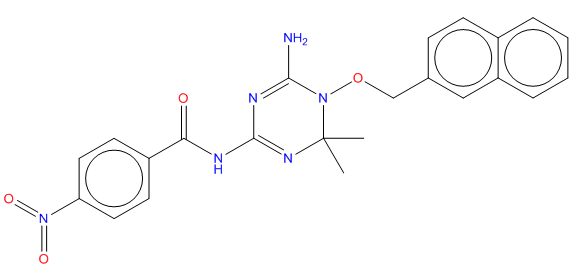
\includegraphics[width=2.5in]{fig/tcam1_mol.png}\\
(b)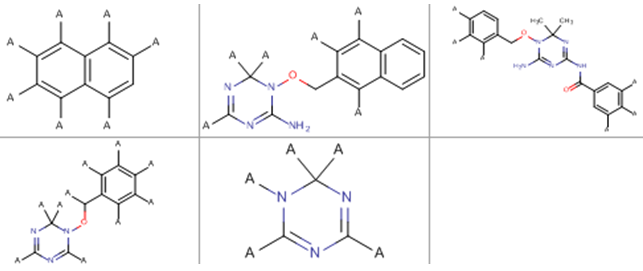
\includegraphics[width=4in]{fig/tcam1_RGscaf.png}\\
(c)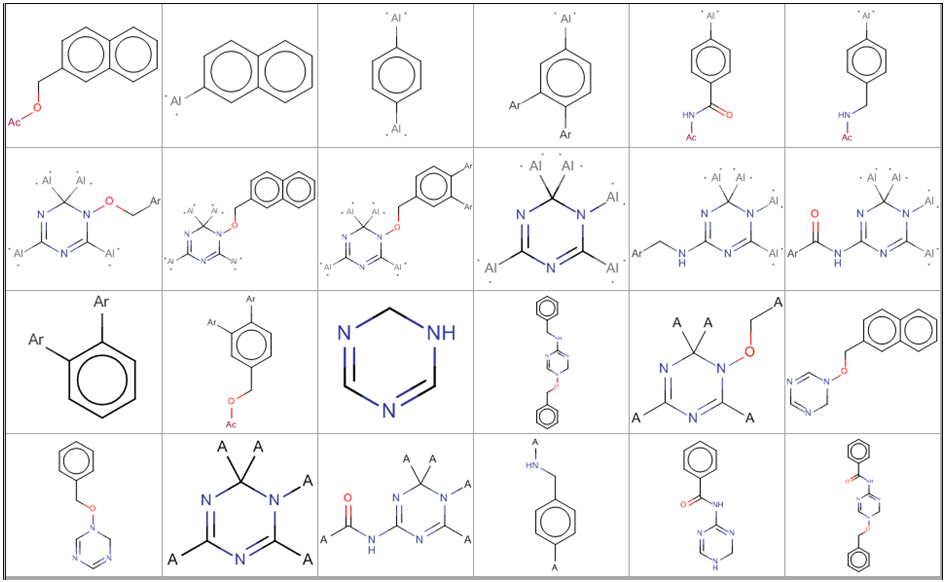
\includegraphics[width=4in]{fig/tcam1_GSKframes.png}\\
(d)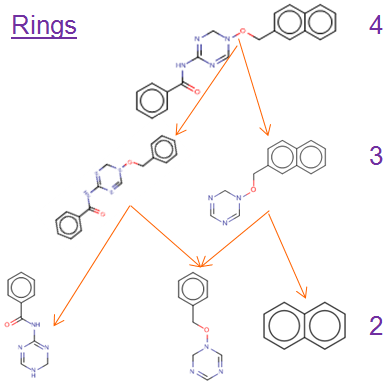
\includegraphics[width=3in]{fig/tcam1_SNG3.png}
\caption{Scaffold Decompositions for a molecule (a) from the TCAMS dataset with PubChem Compound ID 536182. (b) 5 scaffolds from NCATS R-Group Tool; (c) 24 GSK frameworks -- first 21 Bemis-Murcko Like and last 3 in the bottom row RECAP; (d) Scaffold Network generated by SNG, starting from top-level scaffold with four rings down to to all subscaffolds with two rings.}
\label{fig:scafmethod}
\end{figure}

\textbf{\textcolor{red}{NCATS folks, please clarify and fill in any other relevant details}}.

The original NCATS R-group tool focused on scaffold decomposition and
the subsequent generation of R-group tables for each scaffold. Since
then it has been extended to support scaffold hopping as well as
providing contextual data (\eg literature references, activity
summaries) and network visualizations of scaffold relationships. In
this study we employ the latest version (available from
~\url{http://tripod.nih.gov/ws/rgroupbeta/rgrouptool11.jar}). When
running from the command-line, ensuring 16G of memory (via
\texttt{-Xmx16G}) enables datasets of upto ~40k compounds with a
handful of numeric activity columns to be analyzed without running out
of memory. The scaffolds along with R-group tables for each scaffold
can be exported in a set of TSV files or a single JSON file. In the
current work we employed the TSV format which is briefly described.

The scaffold file lists the scaffolds, one to a row with the following
key columns:
\begin{itemize}
\item {\it $Scaffold\_ID$}: Numeric scaffold identifier. Each scaffold occurs only once, and data columns are aggregated for all molecules containing the scaffold.
\item {\it Structure}: Scaffold SMILES without R-groups attached. 
\item{\it RgroupLabels}: A comma separated list of R-group labels for
  all R-groups associated with the scaffold
\item {\it Scaffold Score}: \textbf{Do we want to discuss and define this here?}
\item {\it Complexity}: A number that captures increasing size and complexity of scaffolds - increases with number of rings, non-ring atoms, chiral atoms and ring adjacencies. \textbf{Trung or anyone else, would you like to provide more detail on this and the following scaffold metrics?}. Complexity can be used to prune away scaffolds that are too simple, by setting a cutoff such as 100.  
\item {\it Count}: Number of molecules that share this scaffold
\end{itemize}
The remaining columns are aggregated property columns. Thus for ecah
property of the input molecules, we compute the mean and standard
deviation of that property for all molecules containing the
scaffold. These values are reported in columns labeled \texttt{X} and
\texttt{X_sd}, where \texttt{X} is the property name.

The corresponding R-group decomposition file contains the following columns:
\begin{itemize}
\item {\it ScaffoldID}: Numeric scaffold identifier (corresponding to
  the {\it ScaffoldID} column in the scaffold file
\item {\it MolID}: Numeric or text molecule identifier (name). Each molecule is repeated once for each scaffold that it occurs in.\
\item {\it Structure}: Molecule structure
\item {\it $R_1..R_n$}: R-group SMILES, with \*-atoms at attachment
  points. By default we limit to $n = 21$
\end{itemize}

\subsection{Fragmentation Method: GSK Frameworks}
\label{sec:gskframe}
The R-group Tool described above uses the NCATS implementation of Molecular Frameworks to generate scaffolds. GSK's implementation of Molecular Frameworks is subtly different, and its use has been described in \citeauthor{Harper2004DDclus}. The two types of framework we retain for this study are Bemis-Murcko-like (\cite{BemisMurcko1996} with atom and bond orders retained) and RECAP\cite{Lewell:1998aa}. Other fragmentation methods described by \citeauthor{Harper2004DDclus} such as reduced graphs and classic Bemis-Murcko scaffolds (without atom types and bond orders) were skipped for the purposes of comparison; however there is no reason these could not be included in the framework we are proposing.    

The input for the GSK frameworks code is a comma separated text file
with molecules encoded in a SMILES field.  The code was modified by
adding scripts to export the fuzzy clusters in a tabular format rather
than prioritize them into mutually exclusive scaffolds as in
\citeauthor{Harper2004DDclus}. This step produces a file similar to
the R-group decomposition format described for the NCATS R-group tool
in \sref{rgtool}: framework ID, framework SMILES, molecule ID, SMILES
and replicated property/activity columns.  There are no R-group
columns simply because this is not a default computation in the GSK
frameworks code.

The GSK frameworks found within the same molecule from TCAMS are shown
in \fref{scafmethod}(c).  The reader will observe several differences
from the R-group tool: there are more scaffolds found, some clipped in
the middle of a linker rather than at a ring, and some redundancy
between multiple scaffolds. We will see in Section \ref{sec:results}
that comprehensive coverage of fragments within each molecule can be
both good and bad.

Further details on how to set up and run the GSK frameworks code are
provided in the Supplementary Material.

\subsection{Fragmentation Method: Scaffold Network Generator}
\label{sec:SNG}
The Scaffold Network Generator (SNG) \cite{Matlock2013SNG} is a
parallelizable and robust code to generate a hierarchical Scaffold
Network from any chemical dataset. The operation of this tool is
described on the web at
\url{https://bitbucket.org/swamidass/scaffold-network-generator/wiki/Home}. SNG
takes as input either a SMILES or an MDL SD-file, and we specify
options to generate the Network and ID Map files as two tabular
outputs.

The Network file lists each Scaffold with numeric ID, SMILES, Number
of Rings (which serves as the level in the hierarchy) and Subscaffolds
presented as a comma-separated numeric list. We wrote a script to
split the subscaffold list among multiple lines with the other fields
duplicated, since this format is more amenable to Spotfire integration
as described in a later section.  This script is made available in the
Supplementary Material.

The ID Map file has two columns, mapping a Molecule ID from the primary dataset to the Top-Level Scaffold (i.e. Murcko scaffold) obtained by stripping all pendant groups but no rings. Using the ID Map file followed by multiple iterations of the Network file one can elucidate the entire Scaffold Network starting from each query molecule, as described in a subsequent section.  As an example the scaffold network generated for a molecule from TCAMS is show in \fref{scafmethod}(d), as for the previous two methods.


\section{Methods: Data Integration and Visualization in Spotfire}
\label{sec:methods2}

Next, we describe how tabular scaffold output generated using the
NCATS R-group tool and other comparable methods is integrated into
Spotfire, our visualization tool of choice at GSK.

\subsection{Data Table Generation and Linking}

\begin{figure}
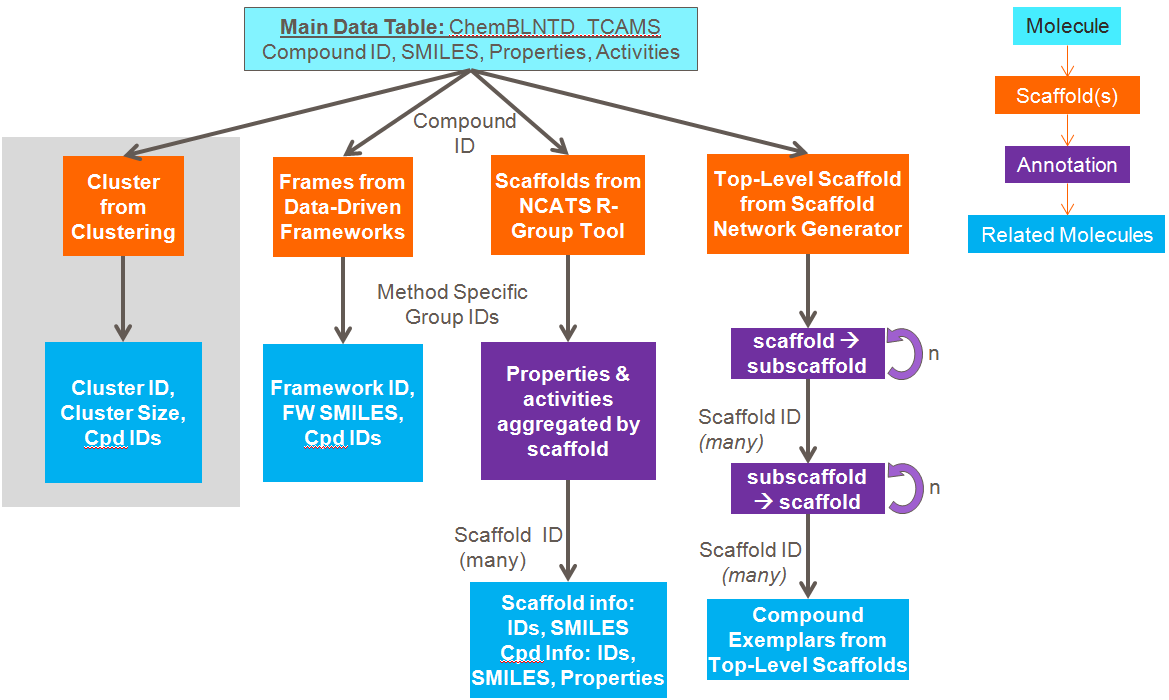
\includegraphics[width=6in]{fig/details_all2.png}
\caption{Detailed schematic on how the output from clustering and fragmentation methods are set up as data tables and linked together with the main dataset in Spofire. Right inset: schematic color-coded view of the scaffold-walking navigation that is loosely followed in this diagram.}
\label{fig:detaildevil}
\end{figure}

\fref{detaildevil} shows how the data tables output by the scaffold generation methods we have considered are layered onto the primary data table in Spotfire. This primary data table is usually a direct import of tabular molecule and activity data generated at GSK or available from public datasets. What gets added is by and large similar, following the framework ``Molecule --> Scaffold (including Annotation) --> Related Molecules'' shown in the figure. For each Molecule in the dataset, we connect it to every Scaffold/Framework/Cluster it contains, and then to every other molecule containing any of these Scaffolds/Frameworks/Clusters. Slight differences for each individual method are detailed below. 

{\bf Complete Linkage Clustering} adds a Cluster Number to the primary data table. To get the Related Molecules, we simply add a duplicate copy of the primary data table and link it to the original via Scaffold ID. In other words, a Table Relation is entered into Spotfire so that $Main.CLink = Main(2).CLink$.  

{\bf GSK Frameworks} are similar to Clusters, except the one-to-many rather than one-to-one mapping of molecules to frameworks. To get the Related Molecules, we add an original and a duplicate copy of this mapping, and set Relations so that:  
\begin{itemize}
\item $Main.Molecule\_ID = Frames(2).Molecule\_ID$
\item $Frames(2).Framework\_ID = Frames.Framework\_ID$
\end{itemize}

{\bf NCATS R-group Tool} adds an additional Annotation layer, \ie the scaffold-level summaries in addition to the R-group decomposition table. In order to enable bidirectional navigation from scaffolds to molecules, we add both these tables and also a duplicate copy of the R-group decomposition table. Then Relations are set up as follows within Spotfire:
\begin{itemize}
\item $Main.Molecule\_ID = RGdecomp(2).Molecule\_ID$
\item $RGdecomp(2).Scaffold\_ID = Scaffolds.Scaffold\_ID$
\item $Scaffolds.Scaffold\_ID = RGdecomp.Scaffold\_ID$
\end{itemize}   

{\bf Scaffold-Network Generator} adds several additional layers of
complexity to the preceding methods. The Molecule ID in the primary
dataset is linked only to the Top-Level Scaffold ID in the ID Map
file; there exists no reverse mapping from subscaffolds with fewer
rings deep within the network to related Molecule IDs. Thus we create
one by assuming one wants to explore at most three levels deeper than
the top level scaffold, but not connect to other molecules that share
only a single ring (rather than a larger system of two or more rings)
with the parent molecule. Thus we add six (three in each direction)
copies of the Scaffold Network table, two of the ID Map table, and two
of the primary data table, connecting them using the following logic:
\begin{itemize}
\item In the three Forward instances of the Network table, the
  Scaffold to Subscaffold Mapping already exists. Modify it by
  truncating (assigning a null subscaffold) when the number of rings
  is 2 or 1.  \subitem Define a new column that maps a null
  subscaffold to the same scaffold, to be able to follow the link to
  downstream tables without diving deeper.
\item In the three Reverse instances of the Network table, the
  Subscaffold to Superscaffold mapping needs to be defined by
  inverting the provided mapping. Thus: \subitem We define in each
  network table a duplicate scaffold ID field, dupID, so that one
  instance of the ID can be used to map in either direction without
  introducing a cycle.  \subitem The mapping from scaffolds in one
  table ($A$) to superscaffolds in one table higher ($B$) is then
  recast as one from scaffolds in $B$ to subscaffolds in $A$, using a
  different set of IDs from the upward links.
\item The Table Relations are then set up as follows to link Molecules
  to Related Molecules in the scaffold network: \subitem
  $Main.Molecule\_ID = ID\_Map(2).Molecule\_ID$ \subitem
  $ID\_Map.Top\_Level\_Scaffold = NetworkDown(3).Scaffold$ \subitem
  $NetworkDown(3).SubScaffold = NetworkDown(2).Scaffold$ \subitem
  $NetworkDown(2).SubScaffold = NetworkDown.Scaffold$ \subitem
  $NetworkDown.Scaffold = NetworkUp.SubScaffold$ \subitem
  $NetworkUp.Scaffold = NetworkUp(2).SubScaffold$ \subitem
  $NetworkUp(2).Scaffold = NetworkUp(3).SubScaffold$ \subitem
  $NetworkUp(3).Scaffold = ID\_Map.Top\_Level\_Scaffold$ \subitem
  $ID\_Map.Molecule\_ID = Related
  Molecules(Copy~of~Main).Molecule\_ID$
\end{itemize}   

We would like to emphasize that the above is one possible engineering solution we found for the problem of linking molecules to related molecules in Spotfire.  Several other solutions have been explored by our colleagues, which include: duplicating columns rather than tables; joining and merging all data into one giant table rather than maintaining multiple linked tables; linking up molecules directly to lists of other molecules in a preprocess that happens outside Spotfire (\eg in a script that integrates the data); and using various add-ins for Spotfire such as the SAR Toolkit{\bf RefBravi} and Discngine {\bf RefDiscngine}.
 
\subsection{Visualization of Molecules, Scaffolds and Related Molecules}

Here we aim to provide one possible minimal and semi-intuitive interface for exploring the network of molecules, the scaffolds they contain and related molecules that contain the same scaffolds. This minimal set consists of the following:
\begin{itemize}
\item {\bf Main Window}: Views defined that allow one to explore the Primary Data Table (with no scaffold information) in the most useful way for each dataset.  The the canonical example, key activity, selectivity, ligand efficiency and molecular properties may be highlighted on the X, Y, shape, size and color axes on a scatter plot. The main window is illustrated for the TCAMS dataset in \fref{spotviz}(a).
\item {\bf Scaffolds and R-groups Tab}: This tab, currently specific to the NCATS R-group tool method for generating scaffolds, contains two visualizations, as illustrated for the TCAMS dataset in \fref{spotviz}(b):  
\subitem The first is a scatter plot display of the Scaffolds table, most commonly with Complexity and Count on the axes and sized by aggregate activity of each scaffold.  Here scaffolds of lesser interest (for example with low complexity or count) can be identified and tagged to remove them from the analysis. Conversely, scaffolds of high interest, for example with many active members or high aggregate ligand efficiency, may be tagged into separate categories.
\subitem The second plot is an R-group table, \ie a Table view of the {RG}decomp table limited to data records that have been marked, \ie molecules that lie in scaffolds currently marked. The table is sorted first by scaffold and then by primary activity, and molecular fields such as Scaffold SMILES, Molecule SMILES and R-groups $R\_1..R\_n$ are rendered using an appropriate depiction package - at GSK this is {JChem}.  This table may be exported to Excel as an on-the-fly R-group table of the scaffolds of interest.
\item {\bf Related Molecules Tab}: The purpose of this tab is to implement the Scaffold Walking navigation described briefly earlier.  The setup is described for the NCATS R-group Tool decomposition, though this tab applies to and can be set up analogously for any of the other decompositions. The tab consists of two visualizations, illustrated for the TCAMS dataset in \fref{spotviz}(c-d):
\subitem The first one is a miniature version of the Main tab, allowing the user to select molecules of interest without flipping over to the Main tab. Doing so drives one of the following two visualizations.
\subitem {\bf Scaffold Trellis}: Visualization on the {RG}decomp table with data limited by the Marking, to only show molecules from the scaffolds the current molecule contains, \ie Related Molecules.  This scatter plot is trellised by Scaffold ID and ideally displays the same properties on the axes as the Main visualization above it.  The trellis allows us to break up the SAR for each constituent scaffold individually, identifying promising scaffolds and substituting unproductive ones as we will describe in the Discussion. The trellis visualization suffers from one redundancy that may be seen in \fref{spotviz}(c): the same molecule occurs in multiple trellis panels and the only way to link them is by X and Y coordinates, by observing groups of points that are laid out similarly across multiple trellis panels.  Though some of our users still prefer this approach, we now describe a newer solution that better leverages Spotfire's capabilities. 
\subitem {\bf Scaffold Pies}: Visualization on the {RG}decomp table with data limited by the Marking, to display Related Molecules as explained above. Instead of using a trellis, the Marker shape is changed to Pies, with Colors (which map to pie sectors) by Scaffold ID, and sectors sized by the Count of molecules in each scaffold.  The setup is illustrated in \fref{spotviz}(d). This plot shows only one point per related molecule but one sector for each scaffold it shares with the parent molecule.  As we'll see later in the Results, this lets the user quickly and visually home in on key substructures that are important or unimportant for activity. 
\end{itemize}

Other visualizations are definitely possible, and in previous iterations of this work we have explored both Box Plots and Cross Tables to summarize the properties of each scaffold beyond the summaries produced by the R-Group Tool -- for example, to explore minimum, maximum, median, most frequent or all values of a field for a particular scaffold.  

In the Supplementary Material we describe some of these alternate visualizations and also describe several Spotfire tricks that are instrumental in making our visualization useful to the chemist or biologist user. 

\subsection{Statistical Comparison of Scaffold Generation Methods}
\label{sec:statmethod}
Our goal in this section is to define the statistical methods that we
have applied in characterizing various methods for classifying
molecules using multiple non-overlapping scaffolds, as opposed to
partitioning the set of molecules into non-overlapping categories
(clusters). The similarities and differences between non-overlapping
ontologies have been analyzed in the literature, and one example is
the method of \citeauthor{Torres2009}, who provide a similarity
measure between outputs of two partitioning clustering methods (not to
be confused with the similarity measure between items that is used to
define the clustering). They use Jaccard's similarity coefficient
$S_{ij}$, defined as the ratio of intersection size to union size of
two groups $i$ and $j$ in the ontology -- similar in spirit to the
Tanimoto coefficient used to define Chemical fingerprint similarity.
This coefficient, computed pairwise and summed, yields a simple
similarity measure between two clusterings $X$ and $Y$ with $m$ and
$n$ members, respectively:
\begin{equation}
Sim(X,Y) = \Sigma_{i \le m, j \le n}{S_{ij} / max(m,n)}
\end{equation}

We adapt this method for SAR analysis using overlapping scaffolds, where the question on the minds of chemists is twofold: what are the fragments in active/desirable molecules, and which other molecules share these fragments? Now if there are two methods $A$ and $B$ of fragmenting compounds, we can evaluate for any molecule how many other molecules share fragments from $A$ or from $B$, and thus can be found using ontologies $A$ alone, $B$ alone, $A$ and $B$, or $A$ excluding $B$.  Using these methods we can evaluate the overall similarity of methods $A$ and $B$, and also independently score the usefulness of $A$ and $B$.

For any compound $C$ and ontology $A$, define the structure group of $C$ under $A$, $C_A$ as the set of compounds that share fragments from $A$ with compound $C$. Similarly define the structure group of $C$ under $B$, $C_B$ as the set of compounds that share fragments from $B$. The Common Proportion ($CP$) for compound $C$ is then defined as the fraction of compounds found by combining both methods that would have been found by either method alone:

\begin{equation}
CP(C) = \| C_A \cap C_B \| / \| C_A \cup C_B \|
\end{equation}

Similar statistics can be defined to rank the usefulness of an individual ontology given others. The Proportion of Information $PI(A)$ calculates the proportion of compounds reachable from $A$ and $B$ that would be reachable from $A$ alone:

\begin{equation}
PI_C(A) = \| C_A \| / \| C_A \cup C_B \|
\end{equation}

In constrast, the Proportion of Information Unique to $A, PIU(A)$ uses the set difference to get at the question: if I have $B$, do I still need $A$? 

\begin{equation}
 PIU_C(A) = \| C_A \setminus C_B \| / \| C_A \cup C_B \| = 1 - PI_c(B)
 \end{equation}
  
When comparing one fragmentation method against another, we often see that one method utilizes a vastly greater number of shared fragments than the other in order to connect compound $C$ to a very similarly sized structure group. To capture this tendency and reward methods that connect molecules to related ones efficiently rather than exhaustively, we define a Fragment Efficiency measure as follows. Let $frag_A(C)$ be the set of fragments of compound $C$ in ontology $A$ that connects $C$ to its structure group $C_A$. Similarly define $frag_B(C)$ for ontology $B$. Then: 
\begin{equation}
FragEff_A(C) = \| C_a \| / \| frag_A(C) \|
\end{equation}


These statistics can be averaged over all compounds in a dataset to yield the Average Common Proportion (ACP), Average Proportion of Information (API), Average Proportion of Information Unique to A (APIU) or Average Fragment Efficiency (AFE).  Other statistics can also be applied to the distribution of $CP$, $PI$ or $PIU$ to characterize the dataset and overlapping scaffolds used to characterize it.

Our methods extend the similarity score of \citeauthor{Torres2009} to
overlapping clusters by using a set of non-overlapping clusters
derived from them, defined as follows:
\begin{itemize}
\item Replace the original clusters by new clusters, one for each item
  in any cluster (in this case, any compound in the dataset).
\item The cluster for Compound $C$ contains all compounds that appear
  with Compound $C$ in any cluster, \ie $C_A$.
\end{itemize}


\section{Results}
\label{sec:results}
Here we illustrate some of our key findings and use cases on a few datasets. 

\subsection{Use Case: Scaffold Progression and Prioritization}
\textbf{Since the current use case is on the GSK Kinase X dataset, this part will have to be approved by GSK legal before placing specific results here. Or we can substitute it.}
To conclude, we have observed how scaffold-based analytics allows us to make decisions based on the aggregate (average, SD, median, min, max, ...) properties of molecules in scaffolds. An entire scaffold may be rejected or prioritized at a time instead of keeping track of individual molecules. It is important to note that rejecting a scaffold does not reject all molecules containing that scaffold - otherwise rejecting the benzene ring would remove a large percentage of valid leads. Also at any time we are able to drill down into the data for individual compounds in interesting scaffolds, whether in an R-group table or a custom plot, and incorporate that into our prioritization.   

\subsection{Use Case: Dataset Fusion and Hybridization}
\textbf{Since the current use case is on the GSK Kinase X dataset, this part will have to be approved by GSK legal before placing specific results here. Or we can substitute it.}
  
To summarize, disparate datasets with no common activity fields (or if preferred, activity fields normalized to a common scale) can be combined and merged at the scaffold level to derive insights such as:
\begin{itemize}
\item Are there regions of chemical space that are unique to one dataset and should be explored further to enrich the chemical diversity available?
\item Conversely, are there chemotypes that substantialy overlap between the datasets?  This might increase confidence in otherwise noisy screening data and provide a coherent SAR picture (including defining series) that might not be available from individual datasets.
\item Can active or otherwise interesting scaffolds from one or a few datasets point to latent or unmeasured actives in other datasets that can then be synthesized (if virtual) or measured (if available) to confirm their activity or add a SAR data point. 
\item If there is a common chemical motif behind several actives, the method will reveal it automatically without relying on a chemist's having seen and flagged the similarity, even if the molecules concerned are disparate looking, few, and scattered across datasets.
\item A cohesive view of actives, inactives, and SAR from a set of screening campaigns helps to summarize the effort and return to it if needed without relying on memory, lab notebooks or manual effort in collating and remining the data.   
\end{itemize} 

\subsection{Use Case: Scaffold Walking Navigation}
\label{sec:scafwalk}
Scaffold Walking is our term for navigating from molecule(s) through scaffolds (implicitly) to Related Molecules. This contrasts with Scaffold Hopping, which is usually defined as a complete replacement of a scaffold by another 2D-dissimilar but 3D-similar or bioisosteric scaffold. Scaffold Walking is meant to be a gradual change to the molecule, at each step retaining at least one element of its maximal Murcko scaffold (\ie at least one among the multiple scaffolds it shares with other molecules in the dataset).  In the process the SAR gets deconvoluted in terms of these scaffolds, allowing us to determine visually both the most essential scaffolds in a molecule and the best Related Molecules containing them.       
\begin{figure}
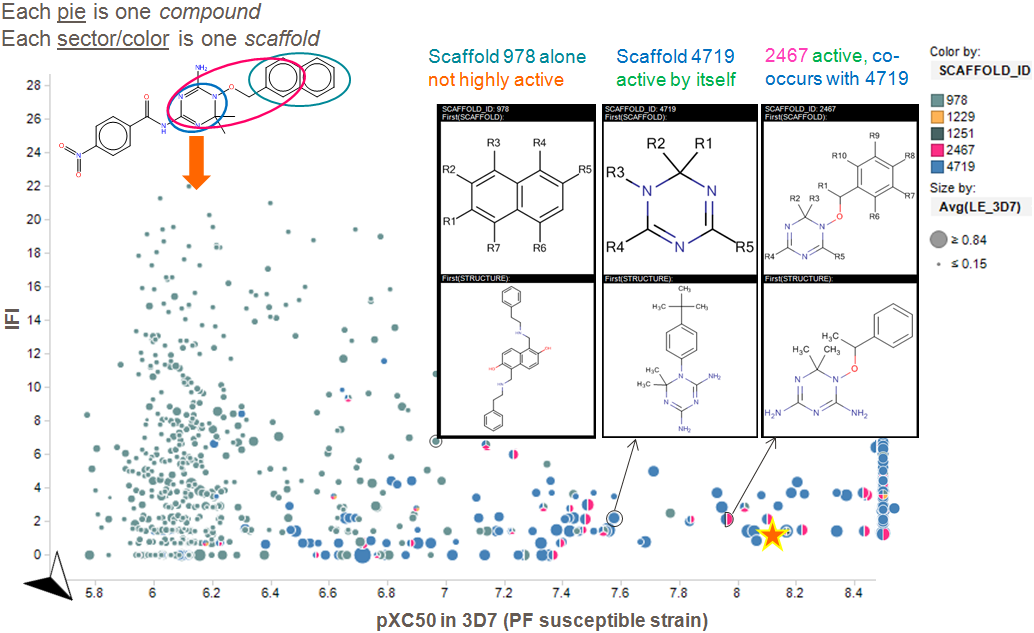
\includegraphics[width=6in]{fig/mol1_RGtool_scafpie.png}
\caption{Related Molecules scaffold pies visualization for Molecule 1 (CID: 536182). Each pie here is one related molecule, and each pie sector and color is a scaffold that it shares with the parent molecule. The star symbol is added to show the location of the parent molecule in this plot, and the compass device at the origin shows the direction of favorable properties (in this case towards the +X and -Y axes). Insights derived from the plot are highlighted in the figure and also discussed in the text.}
\label{fig:scafwalk1}
\end{figure}

As an example, consider Molecule 1 (PubChem CID: 536182) in \fref{scafwalk1}, as a hit that we want to explore SAR of and optimize. This molecule contains 5 scaffolds as determined by the NCATS R-group tool. Using the Scaffold Pie visualization, we observe that the naphthyl scaffold (\#978, cyan) is by itself only moderately active.  The dihydrotriazine (\#4719, blue) scaffold is observed to always occur where the dihydrotriazine-phenethyl-ether (\#2467, pink) one does, implying the substructure relationship between them visually even if one did not know it beforehand. Scaffold \#4719 also exists and is active without \#2467, implying that the phenethyl ether can be substituted and the dihydrotriazine may be sufficient for activity by itself.

\begin{figure}
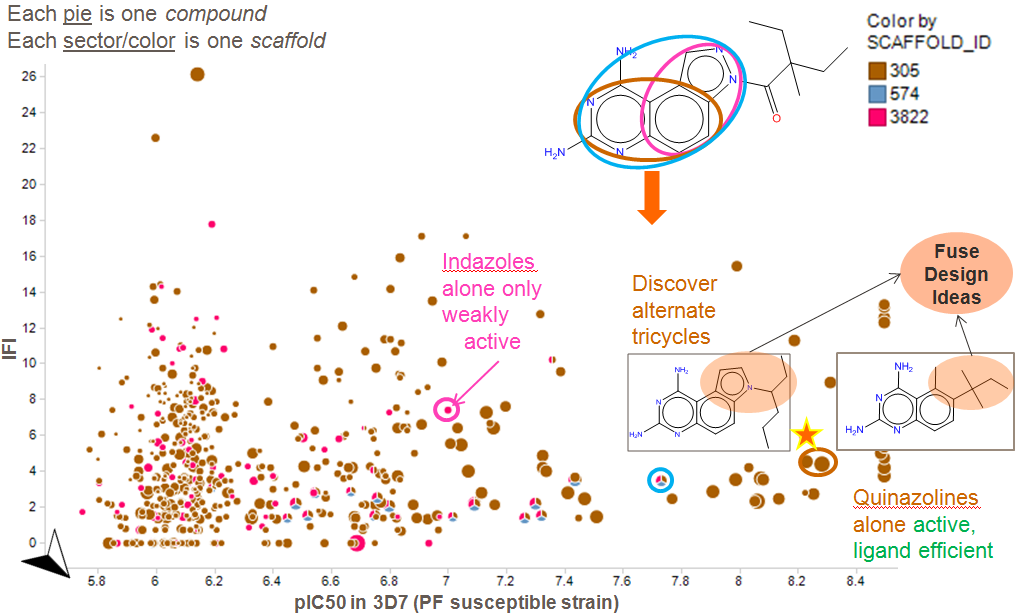
\includegraphics[width=6in]{fig/mol2_RGtool_scafpie2.png}
\caption{Related Molecules scaffold pies visualization for Molecule 2 (CID: 533945). Each pie here is one related molecule, and each pie sector and color is a scaffold that it shares with the parent molecule. The star symbol is added to show the location of the parent molecule in this plot, and the compass device at the origin shows the direction of favorable properties (in this case towards the +X and -Y axes). Insights derived from the plot are highlighted in the figure and also discussed in the text.}
\label{fig:scafwalk2}
\end{figure}

Molecule 2 in \fref{scafwalk2} is another case where we might want to optimize the physical and chemical properties of the molecule without sacrificing activity or increasing promiscuity. Since solubility has been shown to go down with number of aromatic rings independent of lipophilicity\cite{Hill2010}, walks that remove one or more of the three fused rings might be productive. By exploring the Related Molecules, we observe the SAR for three scaffolds: quinazolines (\#305, brown), indazoloquinazolines (\#574, blue) and indazoles (\#3822, pink). We observe from the plot a few more molecules containing all three scaffolds (tricolored pies, \ie exact analogs of the parent molecule); all of these are less active than the parent. The indazoles when they occur alone (pink circles) are far less active than the parent, suggesting they do not contribute significantly to activity and may be substituted. Lastly the quinazolines (brown) include several analogs that are more active and also less promiscuous than the parent. Drilling down into these structures, we observe several that contain only two aromatic rings (\ie no more are either fused or attached); these provide novel, active and ligand-efficient templates on which to build new analogs with enhanced solubility or other properties. Suggestions for which analogs to make can often be obtained by examining the SAR -- for example, disparate aliphatic and aromatic analogs at two adjacent positions on the quanazoline phenyl are active, which suggests hybridizing them or designing further analogs substituted at these positions.

Another intriguing result is seen by observing a new tricyclic series that shares the quinazoline but adds an indole instead of indazole as the third fused ring. This alternative tricyclic template, while it may not confer solubility advantages, opens up a new area of chemical space. By iteratively seeking the Related Molecules for this new hit as shown in \fref{scafwalk3}, we observed that most of the active quinazoline analogs have this new tricyclic scaffold (\#1824, tan wedges in tricolored pies) and relatively few contain only quinazolines (\#305, brown circles). Also, indoles by themselves (\#1188, blue circles) do not much better than indazoles, so this is a new synergistic effect discovered by scaffold walking from the original hit.            

\begin{figure}
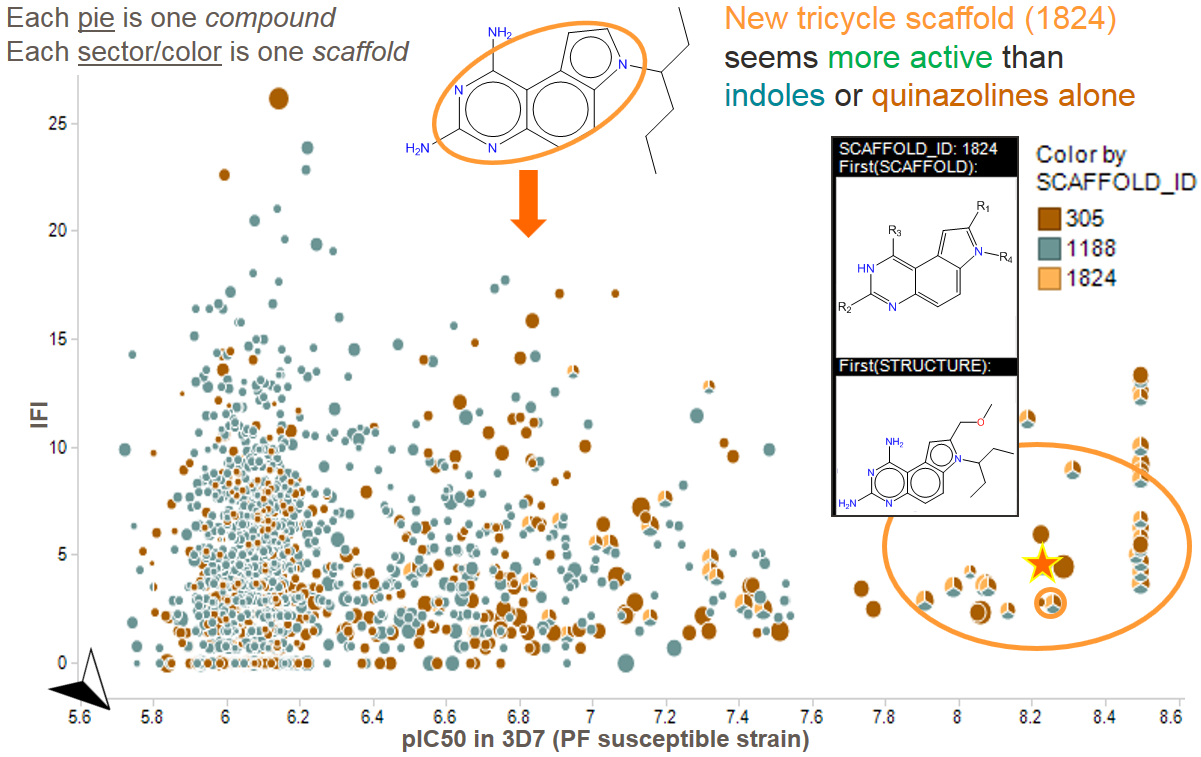
\includegraphics[width=6in]{fig/mol3_RGtool_scafpie_iter.png}
\caption{Iterative Related Molecules scaffold pies visualization for Molecule 3 (CID: 541531), a scaffold hop from Molecule 2 shown in \fref{scafwalk2}. Each pie here is one related molecule, and each pie sector and color is a scaffold that it shares with the parent molecule. The star symbol is added to show the location of the parent molecule in this plot, and the compass device at the origin shows the direction of favorable properties (in this case towards the +X and -Y axes). Insights derived from the plot are highlighted in the figure and also discussed in the text.}
\label{fig:scafwalk3}
\end{figure}

\subsection{Qualitative Comparison of Scaffold-Generation Methods and Clustering}
{\bf Complete-Linkage Clustering}: As shown in \fref{clusterlanes}, the defining feature of a partioning clustering is that every molecule maps to one and only one cluster. Thus if a chemotype is broken up among two or more clusters, using the cluster ID to map Related Molecules can retrieve only neighbors from the same cluster, ignoring the other cluster. This is not ideal for purposes of the visualization and navigation method presented here, as arbitrary neighbors would be excluded depending on how the clustering is defined.  Thus we do not advocate the use of clustering, unless it is a fuzzy clustering where all meaningful class memberships a molecule might have are considered. 

\begin{figure}
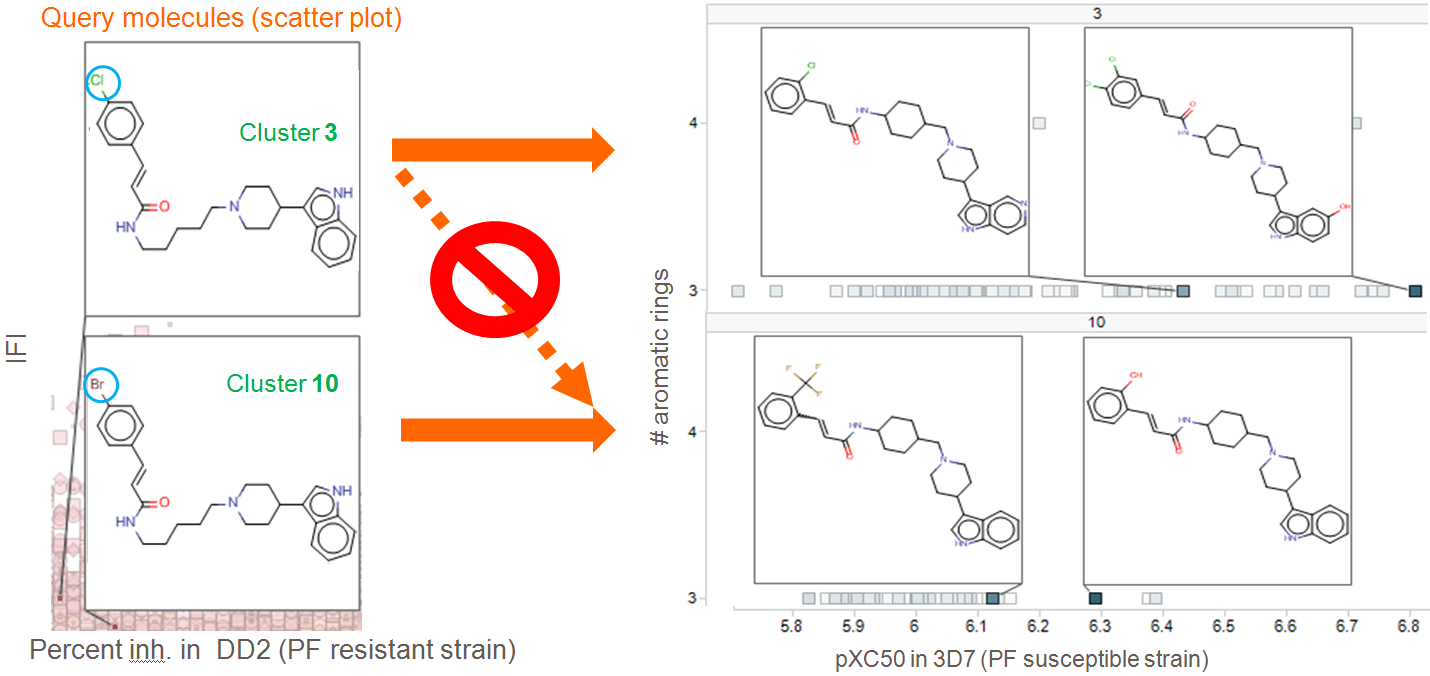
\includegraphics[width=6in]{fig/clusterlanes.png}
\caption{Illustrating one problem with clustering: bifurcation of related molecules.  When two molecules of the same chemotype differing by a halogen are split across Complete Linkage Clusters, searches of cluster neighbors for one molecule do not find its analogs in the other cluster, \ie the two related clusters are not linked.}
\label{fig:clusterlanes}
\end{figure}



{\bf NCATS R-group tool}: As opposed to the clustering method, 
if any two molecules share a common substructure that meets the standards required of a scaffold by the NCATS method (\eg being bordered by rings on each end), then those molecules will be found to contain that shared substructure as a scaffold and their activities will be used to compute aggregate properties for it. 

{\bf Other Scaffold Generation Methods}: As shown above, even though other scaffold generation methods (GSK frameworks and Scaffold Network Generator) differed in their implementation details and produced different numbers of scaffolds for the same molecule, they were roughly equivalent in a qualitative sense with regard to the insights obtained. Due to substantial overlap between sets of scaffolds, ring systems responsible for activity of a molecule were generally revealed by any of the methods. For example, the insights mentioned in \sref{scafwalk} were more or less consistent across the three methods. However, there were cases where the Frameworks revealed negative information about a fragment being not important for activity that is also useful for a drug discovery scientist. For example, in \fref{frameswalk} a substructure is highlighted that is on the aggregate inactive and could be removed or substituted. This insight is not available from the other methods since they don't define or find that fragment as a scaffold.

\begin{figure}
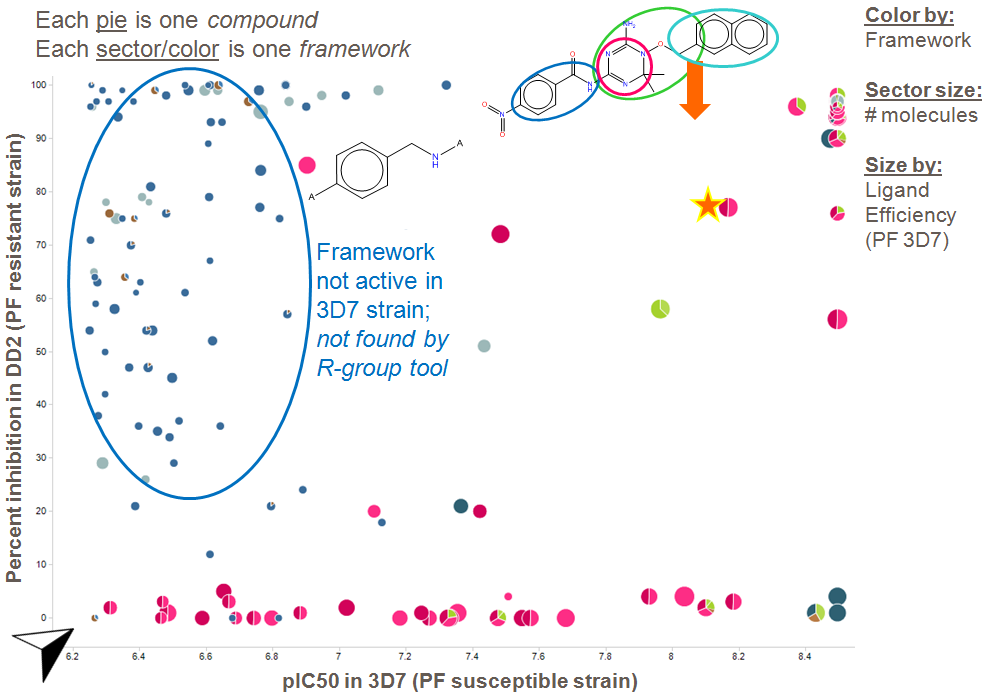
\includegraphics[width=6in]{fig/mol1_frames_scafpie.png}
\caption{Using GSK Frameworks instead of NCATS R-group tool in the Scaffold Pies visualization. One framework is highlighted that has no equivalent in the NCATS scaffolds, but is shown on the average to reduce activity since related molecules that contain it are less active than the parent molecule.   The star symbol is added to show the location of the parent molecule in this Related Molecules plot, and the compass device at the origin shows the direction of favorable properties (in this case towards the +X and +Y axes).}      
\label{fig:frameswalk}
\end{figure}

\begin{figure}
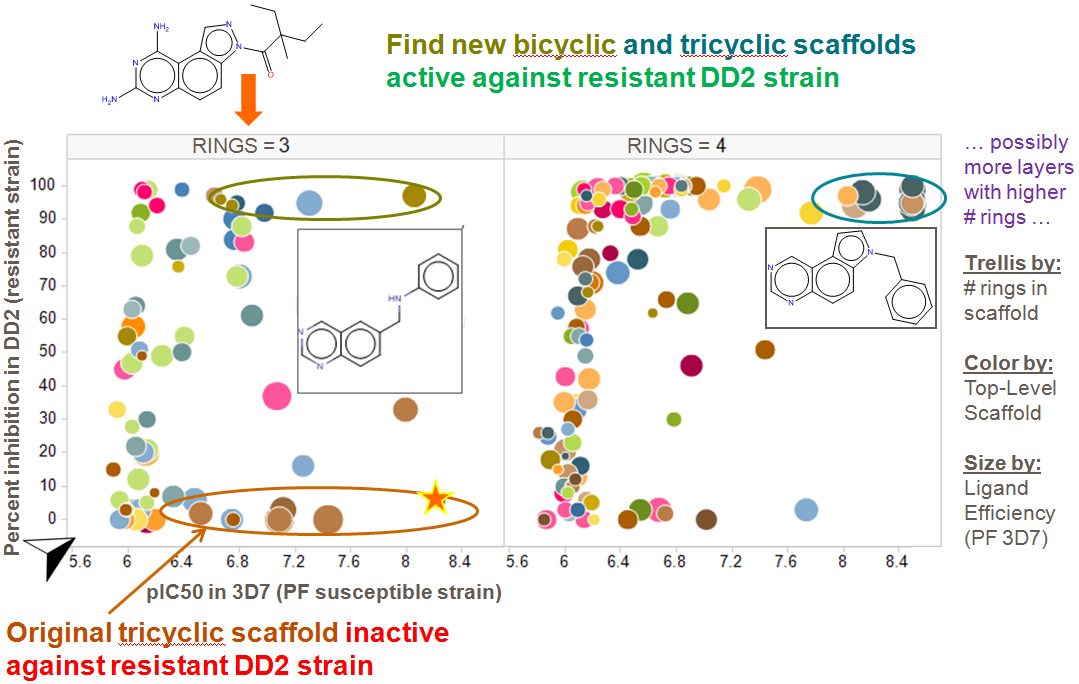
\includegraphics[width=6in]{fig/mol2_SNG_relmol_trellis.png}
\caption{Using Scaffold Network Generator to find Related Molecules a few hops away in the Scaffold Network that have a desirable property, in this case activity against the resistant DD2 strain of P.~falc.  The star symbol is added to show the location of the parent molecule in this plot, and the compass device at the origin shows the direction of favorable properties (in this case towards the +X and +Y axes).}
\label{fig:SNGwalk}
\end{figure}



Using the Scaffold Network to visualize Related Molecules, one is able to deconvolute scaffolds with different numbers of rings (which serves as the level in the hierarchy) by trellising on it, and thus gather together substructures of comparable size. As shown in \fref{SNGwalk}, with the same tricyclic molecule as in \fref{scafwalk2}, we use Scaffold Networks to solve a selectivity issue. Members of the original scaffold, shown in light brown, tend to have some activity against the susceptible 3D7 strain of $P.~falciparum$ but be inactive against the multidrug-resistant DD7 strain. Using the scaffold network to go one level down (to molecules with two rings) and then two levels up (up to 5 rings) we obtain many new molecules that are a few hops away from the top-level tricyclic scaffold while still sharing some aspect of it. Looking at where these new Related Molecules are placed, we mark one scaffold with 3 rings that has a quinazoline linked to a phenyl, and one with 4 rings that contains an indoloquinazoline (also discovered by scaffold walking with the NCATS R-group tool as described above) linked to a phenyl. These two scaffolds are highlighted since their members consistently have high activity against the resistant DD2 strain, and thus this would be a desirable scaffold hop (or walk) towards chemical space that is more useful in overcoming resistance from the malarial parasite.  

To summarize, all three multiple-scaffold decomposition methods considered in this study, \ie NCATS R-group Tool, GSK Frameworks  and Scaffold Network Generator give comparable insights when exploring the TCAMS dataset, with some differences stemming from individual substructures that are considered shared scaffolds or not by the individual methods.  We now explore these overlaps, similarities and differences in the aggregate using the statistical methods described earlier in \sref{statmethod}.

\subsection{Statistical Comparison of Scaffold-Generation Methods}\ref{statcomp}

Recall the concepts of structure group and common proportion defined in \sref{statmethod}.  Let us now apply these to analyze and compare the scaffold generation methods GSK Frameworks ($A$) and NCATS R-group tool ($B$). As an illustration, \fref{strucgroup} (a)-(c) shows the structure group of the compound $C$ with PubChem ID 536182. 
\begin{figure}
  (a)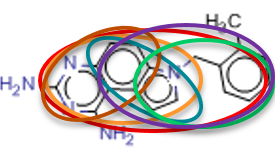
\includegraphics[width=1in]{fig/mol_6scaf.png}
  (b)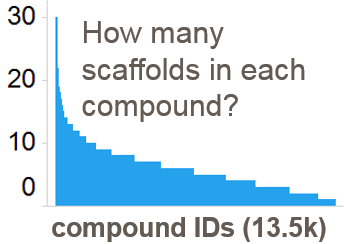
\includegraphics[width=1in]{fig/howmany_scaf.png}
  (c) 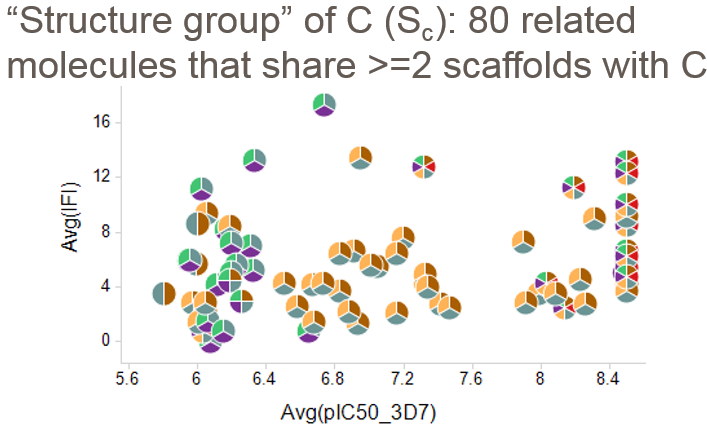
\includegraphics[width=3in]{fig/structure_group_C.png}
  \caption{(a) Compound $C$, chosen here as PubChem ID 536182 from previous figures, has 6 fragments derived using the NCATS R-group tool. (b) Distribution of number of fragments, out of nearly 6000 total, found in each molecule. (c) Scaffold pie plot showing the structure group of $C$, restricted here to only compounds that share two or more substructures with $C$. This ensures that all compounds sharing just a single heteroaromatic ring are not in the same group, as chemists expect, and also reduces the group size -- 80 related molecules for this particular compound $C$.}
    \label{fig:strucgroup}
\end{figure}

We compare the Common Proportion, Proportion of Information Unique (PIU) and Fragment Efficiency (FragEff) statistics for the GSK Frameworks (method ``A'') and the NCATS R-group tool (method ``B'') for all the 13.5k compounds in TCAMS in \fref{statcompare}.  This figure has PIU of methods $A$ and $B$ on the axes, is sized by ratio of Fragment Efficiencies for all 13.5k molecules.   



\begin{figure}
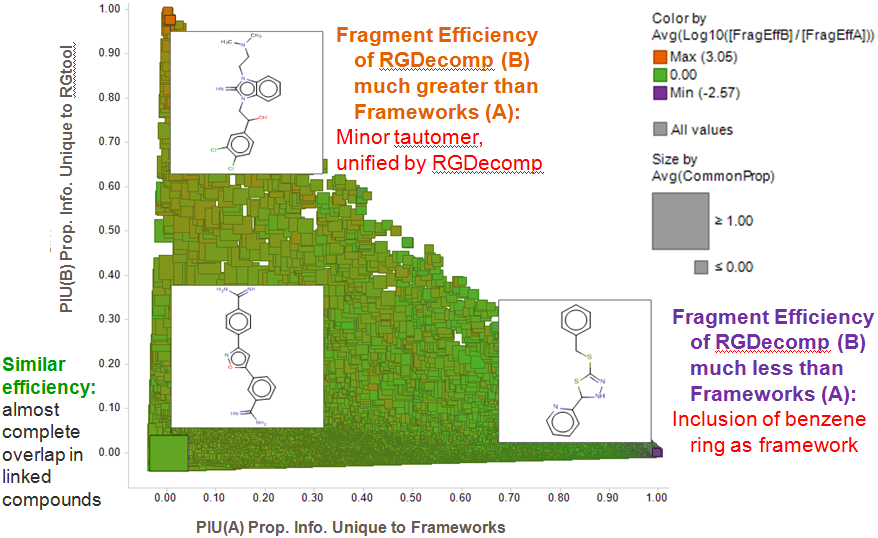
\includegraphics[width=6in]{fig/statcompare_frames_RGtool.png}
\caption{Comparison of the Common Proportion, PIU and FragEff statistics (described in the text) between GSK Frameworks (method ``{\bf A}'') and NCATS R-group Tool (``{\bf B}'') for all molecules in TCAMS. PIU of A and B are on the X and Y axes, and the points are colored by the log ratio of FragEff(B) to FragEff(A) and sizes by Common Proportion.}
\label{fig:statcompare}
\end{figure}
 
Comparing the GSK Frameworks and NCATS R-Group Tool for the TCAMS dataset using the above mentioned statistical metrics, we show the aggregate statistics over the entire dataset in \tref{statcomparetable}.

We can make a few observations from this data and plot:
\begin{enumerate} 
\item The two methods allow one to access different sets of molecules starting from any molecule in TCAMS - the average overlap in their coverage is 40\%.
\item On the average, one can link to about twice as many molecules with the GSK frameworks; however, this is because on the average there are 6 times more frameworks than NCATS scaffolds, so the fragment efficiency is actually 3 times greater for NCATS scaffolds. One could also argue that many of the framework-only links (eg. variously decorated benzene rings) are not useful.
\item The outliers are interesting. At one end, compounds in a rare tautomer are unified with the dominant one by the NCATS tool (high fragment efficiency), but left as singletons by the frameworks (low fragment efficiency). And compounds whose only link with other molecules would be a benzene ring or similar low complexity scaffold remain singletons with the R-group tool (lower fragment efficiency).
\end{enumerate}


\section{Discussion}
\label{sec:discussion}

\begin{itemize}
\item Discuss performance - scaffold generation is usually a one time procedure
  for a given screening deck. Furthermore, the scaffold generating process will
  associate compounds with scaffolds, so looking up scaffold membership is very
  fast. When considering scaffold similarity, usual performance bottlenecks
  occur, same as for other similarity applications. Can we include some
  performance numbers?
\item we haven't discussed removal of promiscuous compounds/chemotypes,
  undesirable chemotypes (ie PAINS etc), these are generally a separate and
  independent step from the scaffold identification process
\item Ranking scaffolds is a key step in prioritizing hits in a scaffold-based
  approach. Still a subjective issue and many ways to do it. Not clear that
  there is a single optimal way. Discussion points could include
  \begin{itemize}
  \item Size and complexity - depending on the application (and
    dataset) smaller scaffolds maybe more relevant or useful than
    larger scaffolds. Scaffold key approach \cite{Ertl:2014eu}
    quantifies this aspect. In some scenarios, the dataset may consist
    of small scaffolds in general (\eg fragment screening
    libraries). Complexity may also play a role in the practicality of
    using a scaffold - highly complex scaffolds may not be easily
    synthesizable or purchasable.
  \item Promiscuity of the scaffold (does it show up in many active
    compounds across different assays?) itself or do the scaffold
    members, in aggregate, show high degree of promiscuity?
  \item Do the members of a scaffold represent a SAR (``SARability'')?
    Could be characterized quantitatively, but such approaches would
    be hampered by the size of the member set. Larger scaffolds will
    tend to have fewer members.  Alternatively, characterize the
    activity landscape of the scaffold member set - overly smooth or
    overly rough landscapes are not useful. But still tricky to decide
    what a sufficiently smooth (or rough) landscape is.
  \item Alternatively, in absence of SAR, does a given scaffold show
    an enrichment of activity (or just actives) compared to other
    scaffolds (after having taken parent-relationships in to account -
    similar to GO enrichment analyses).
  \end{itemize}
\item Privileged scaffolds - sometimes could go in looking for them,
  but usually one identifies such privileged scaffolds in a
  retrospective fashion, across multiple HTS campaigns. Relevance /
  importance to scaffold based triage?
\item The last point also suggests that intuition and experience play
  an important role and also present a possible source of bias. A
  chemist with a ``favorite'' scaffold may (unconciously) tend to
  ignore other scaffolds. To combat such human biases, data driven
  summaries and navigation are vital
\end{itemize}

\begin{acknowledgement}
  The GSK authors thank Subhas Chakravorty, Neysa Nevins, Ami Lakdawala Shah,
  Eric Manas, Todd Graybill, Stan Martens, Mike Ouellette, Tony Jurewicz and Rob
  Young for valuable feedback and suggestions while developing the method and
  visualizations.
\end{acknowledgement}

%%%%%%%%%%%%%%%%%%%%%%%%%%%%%%%%%%%%%%%%%%%%%%%%%%%%%%%%%%%%%%%%%%%%%
%% The same is true for Supporting Information, which should use the
%% suppinfo environment.
%%%%%%%%%%%%%%%%%%%%%%%%%%%%%%%%%%%%%%%%%%%%%%%%%%%%%%%%%%%%%%%%%%%%%
\begin{suppinfo}
Supplementary material is available online for this article.
\end{suppinfo}

%%%%%%%%%%%%%%%%%%%%%%%%%%%%%%%%%%%%%%%%%%%%%%%%%%%%%%%%%%%%%%%%%%%%%
%% The appropriate \bibliography command should be placed here.
%% Notice that the class file automatically sets \bibliographystyle
%% and also names the section correctly.
%%%%%%%%%%%%%%%%%%%%%%%%%%%%%%%%%%%%%%%%%%%%%%%%%%%%%%%%%%%%%%%%%%%%%
\bibliography{bibliography}

\end{document}
